% Projekt: IFJ15 (Interpret jazyka) - dokumentace
% Autor: Patrik Jurnečka
% Login: xjurne03
% Email: xjurne03@stud.fit.vutbr.cz
% Datum: 

\documentclass[a4paper, 11pt, titlepage]{article}
% Preambule
\usepackage[left=2cm, text={17cm, 24cm}, top=3cm]{geometry} %Rozmery
\usepackage{times} %Styl jazyka
\usepackage[IL2]{fontenc}
\usepackage[czech]{babel} %Jazyk
\usepackage[utf8]{inputenc} %Kodovani
\usepackage{graphics}
\usepackage{picture} 
\bibliographystyle{czplain}

\providecommand{\uv}[1]{\quotedblbase #1\textquotedblleft} %Uvozovky 

\begin{document} %Textova cast

\begin{titlepage} %Titulni strana
\begin{center}
\textsc{\Huge{Vysoké učení technické v~Brně}\\[3mm]\huge{Fakulta informačních technologií}}\\

\vspace{\stretch{0.2}}

\begin{figure}[h]
	\centering
	\scalebox{0.11}{\includegraphics{FIT_barevne_RGB_CZ.png}}
\end{figure}

\vspace{\stretch{0.182}}
\huge{Dokumentace projektu do předmětu IFJ a IAL}\\
\Huge{\textbf{Interpret jazyka IFJ15}}\\
\LARGE{Tým 043, varianta b/2/I}
\vspace{\stretch{0.618}}
\end{center}

{\noindent\Large \hfill Martin Honza (xhonza03) - \%\\}
{\indent\Large \hfill Patrik Jurnečka (xjurne03) - \%\\}
{\indent\Large \hfill Hana Slámová (xslamo00) - \%\\}
{\indent\Large \hfill Frantisek Šumšal (xsumsa01) - \%\\}
{\indent\Large\today \hfill Adam Švidroň (xsvidr00) - \%}

\end{titlepage}

\tableofcontents

\newpage

\section{Úvod} %Uvod
Dokumentace popisuje návrh a implementaci projektu Interpret jazyka IFJ15 do předmětu IFJ (Formální jazyky a~překladače) a IAL (Algoritmy). Vybrali jsme si zadání b/2/I, které nám udávalo, jáký algoritmus máme pro daný problém využít. Pro vyhledávání \textbf{Boyer-Mooreův algoritmus}, pro řazení algoritmus \textbf{Heapsort}, který byl využit ve vestavěné funkci \textbf{sort}. Poslední ze specifikových pravidel použití, jsme měli využít k implementaci tabulky symbolů \textbf{binární vyhledávací strom}. 

Cílem projektu bylo vytvořit program, který interpretuje jazyk IFJ15, což je velmi zjednodušenou podmnožinou jazyka C++11. 

\newpage

\section{Struktura projektu}
Překladač je rozdělen do tří hlavních celků. Pomocí \textbf{lexikálního analyzátoru} načítá zdrojový kód. \textbf{Syntaktický analyzátor} zažádá lexikální o token a ověří syntaxi. Po bezchybné kontrole se spustí \textbf{interpret} s kontrolou sémantiky jazyka.  

\section{Lexikální analizátor (scanner)}
Analyzátor je implementován v souborech \textit{lex.c} a \textit{lex.h}. Lexikální analyzátor načítá zdrojový kód po znacích a~převádí jej na tokeny. Veškerá komunikace s dalšími knihovnami probíhá pomocí funkce \textit{lex\_get\_token}. Analyzátor je implementován pomocí konečného automatu (Obrázek~\ref{picture_1:konecny_automat}), přičemž veškeré komentáře ve zdrojovém kódu ignoruje. Funkce je volána vždy, když syntaktický analyzátor zažádá o~token. 

Načítání znaků zajišťuje funkce \textit{fgetc()}. Na základě načteného lexému se rozhodne o jaký typ tokenu se jedná. V některých případech je potřeba načtený znak vrátit do souboru pomocí funkce \textit{ungetc()}.

Token definuje jednotlivé prvky kódu a určuje jak se k němu má při překladu přistupovat. Analyzátor prochází tabulku klíčových slov (\textit{lex\_kw\_t keywords[]}), zda-li nejde o rezervované klíčové slovo pro speciální funkci.

\subsection{Konečný automat}

\begin{figure}[h]
	\centering
	\scalebox{0.23}{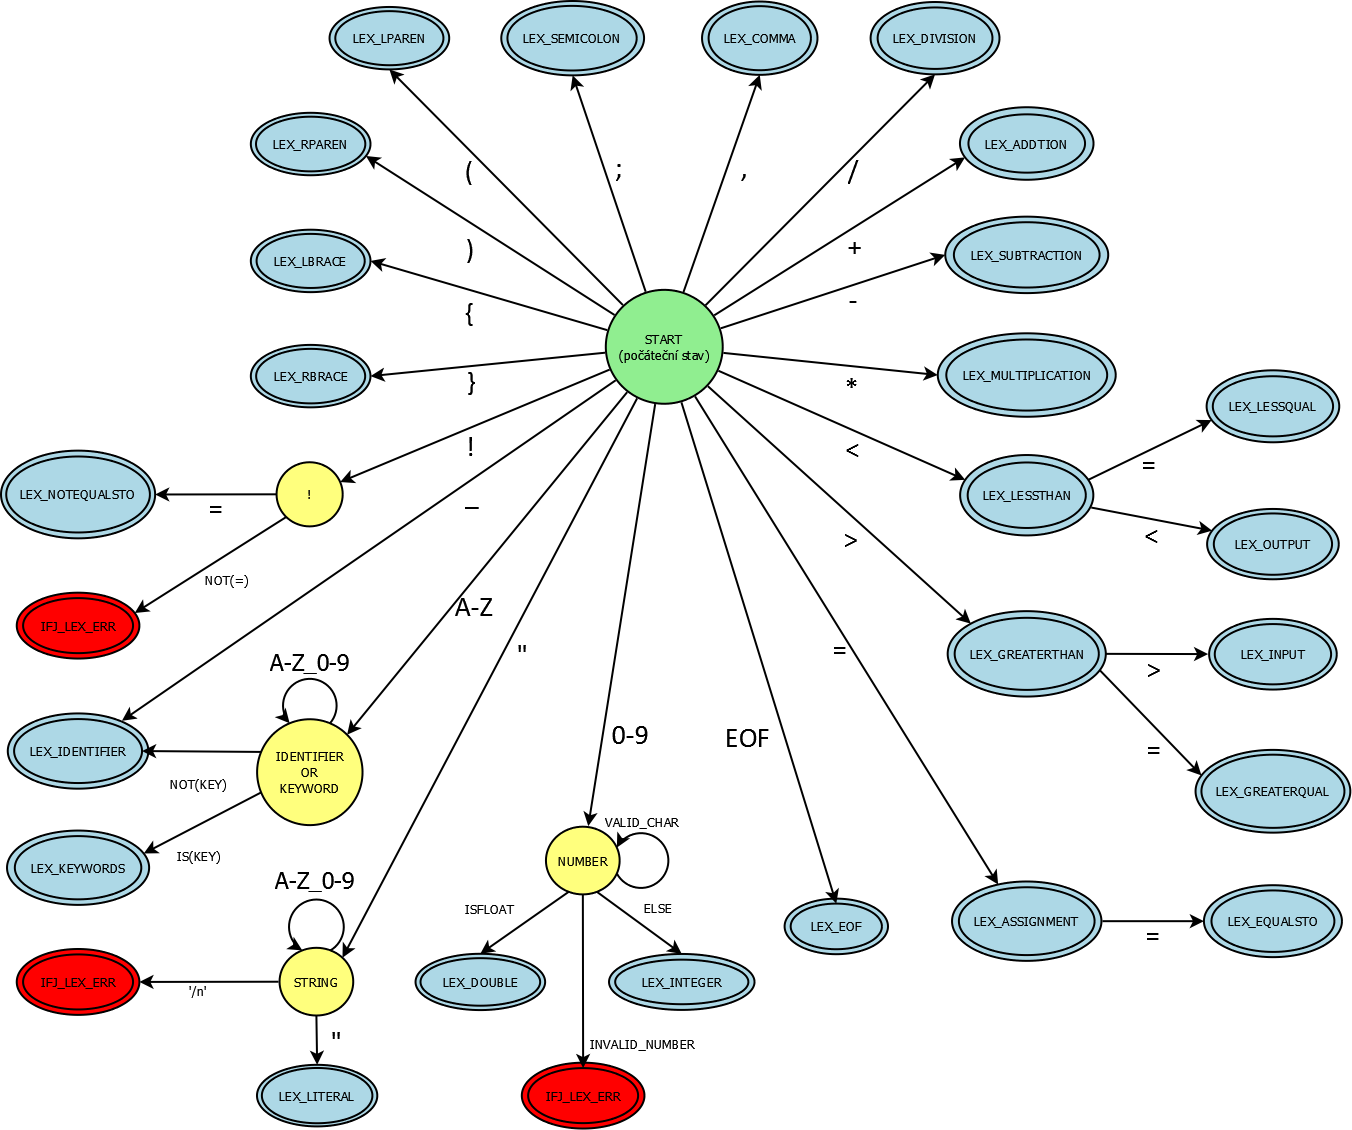
\includegraphics{konecny_automat.png}}
	\caption{Konečný automat}
	\label{picture_1:konecny_automat}
\end{figure}

\newpage
\section{Syntaktická analizátor (parser)}
Syntaktický analyzátor kontroluje syntaktickou správnost zdrojového kódu. Postupně volá tokeny z lexikálního analyzátoru, které jsou zpracovávaný dvěma způsoby. Pomocí LL gramatiky (Tabulka \ref{table_1:LL_gramatic}) a precedenční syntaktické analýzy (Tabulka \ref{table_2:PA}), které jsou jádrem celého SA. Při úspěšném dokončení syntaktické analýzy se generuje instrukční páska pro interpret.

\subsection{Obecný syntaktický analyzátor (LL gramatika)}
LL gramatika postupně ověřuje rekurzivním sestupem příchozí tokeny. Funkce jsou navrženy tak, aby ověřili aktuální token nebo požádali lexikální analyzátor, funkcí \textit{lex\_get\_token} o následující. Nedá-li se rozhodnout na základě pouze jednoho tokenu zažádá si o další.     

\begin{table}[h]
	\begin{center}
	\begin{tabular}{|c| l c l|}	\hline
	1. 	& $<$program$>$       &$ \rightarrow $& $<$declrList$>$ EOF \\
	2. 	& $<$declrList$>$     &$ \rightarrow $& $<$funcDeclr$>$ $<$declrList$>$ $|$ EPSILON \\
	3. 	& $<$funcDeclr$>$     &$ \rightarrow $& $<$typeSpec$>$ ID ( $<$params$>$ ) $<$funcStmt$>$ \\
	4. 	& $<$funcStmt$>$      &$ \rightarrow $& $<$compoundStmt$>$ $|$ ; \\
	5. 	& $<$params$>$        &$ \rightarrow $& $<$paramItem$>$ $|$ EPSILON \\
	6. 	& $<$paramItem$>$     &$ \rightarrow $& $<$typeSpec$>$ ID , $<$paramItem$>$ $|$ $<$typeSpec$>$ ID \\
	7. 	& $<$typeSpec$>$      &$ \rightarrow $& int $|$ double $|$ string \\
	8. 	& $<$statement$>$     &$ \rightarrow $& $<$compoundStatement$>$ $|$ $<$ifStmt$>$ $|$ $<$forStmt$>$ $|$ \\ 	
		& 					  & 			  & $<$assignEndStmt$>$ $|$ $<$callStmt$>$ $|$ $<$returnStmt$>$ $|$ \\  
		&					  &				  & $<$inputStmt$>$ $|$ $<$outputStmt$>$ $|$ $<$varDeclr$>$ $|$ \\ 
		& 					  & 			  &$<$expressionStmt$>$ \\
	9.  & $<$compoundStmt$>$  &$ \rightarrow $& { $<$stmtList$>$ } \\
	10. & $<$stmtList$>$      &$ \rightarrow $& $<$statement$>$ $<$stmtList$>$ $|$ EPSILON \\
	11. & $<$varDeclr$>$      &$ \rightarrow $& $<$typeSpec$>$ $<$varDeclrItem$>$ ; $|$ auto $<$varInitialize$>$ ; \\
	12. & $<$varDelcrItem$>$  &$ \rightarrow $& ID $|$ $<$varInitialize$>$ \\
	13. & $<$varInitialize$>$ &$ \rightarrow $& ID $=$ $<$expression$>$ \\
	14. & $<$ifStmt$>$        &$ \rightarrow $& if ( $<$expression> ) $<$compoundStmt$>$ else $<$compoundStmt$>$ \\
	15. & $<$forStmt$>$       &$ \rightarrow $& for ( $<$varDeclr$>$ ; $<$expression$>$ ; $<$assignStmt$>$ ) \\ 
		& 					  & 			  & $<$compoundStmt$>$ \\
	16. & $<$assignEndStmt$>$ &$ \rightarrow $& $<$assignStmt$>$ ; \\
	17. & $<$assignStmt$>$    &$ \rightarrow $& ID $=$ $<$expression$>$ $|$ ID $=$ $<$call$>$ \\
	18. & $<$callStmt$>$      &$ \rightarrow $& ID $=$ $<$call$>$ \\
	19. & $<$call$>$          &$ \rightarrow $& ID ( $<$callParams$>$ ) \\
	20. & $<$callParams$>$    &$ \rightarrow $& $<$callParam$>$, $<$callParams$>$ $|$ $<$callParam$>$ $|$ EPSILON \\
	21. & $<$callParam$>$     &$ \rightarrow $& ID $|$ LITERAL \\
	22. & $<$returnStmt$>$    &$ \rightarrow $& return $<$expression$>$ ; \\
	23. & $<$inputStmt$>$     &$ \rightarrow $& cin $\gg$ ID $<$inputArgs$>$ ; \\
	24. & $<$inputArgs$>$     &$ \rightarrow $& $\gg$ ID $|$ EPSILON \\
	25. & $<$outputStmt$>$    &$ \rightarrow $& cout $\ll$ $<$callParam$>$ $<$outputArgs$>$ ; \\
	26. & $<$outputArgs$>$    &$ \rightarrow $& $\ll$ $<$callParam$>$ $|$ EPSILON \\ \hline
	\end{tabular}
	\caption{LL gramatika}
	\label{table_1:LL_gramatic}
	\end{center}
\end{table}

\newpage

\subsection{Syntaktický analizátor výrazů (precedenční syntaktická analýza)}
Syntaktická analýza zdola nahoru. Dle Zadání jsme analýzu implementovali za pomocí precedenční tabulky (Tabulka \ref{table_2:PA}) a~níže uvedenou gramatikou, která nám slouží k vyhodnocení vstupních výrazů. Podle zadání projektu jsme vytvořili precedenční tabulku ze zadaných priorit operátorů. SA výrazů je volán vždy, když obecný SA narazí na výraz. Funkce si ukládá jednotlivé příchozí tokeny na zásobník a poté je v závislostí na prioritách jednotlivých prvků vyhodnocuje. 

\begin{table}[h]
	\begin{center}
		\begin{tabular}{l l l l l l}
			E $ \rightarrow $ id & E $ \rightarrow $ (E) & E $ \rightarrow $ E $ \ast $ E & E $ \rightarrow $ E $ \div $ E & E $ \rightarrow $ E$ + $E & E $ \rightarrow $ E$ - $E \\
			E $ \rightarrow $ E $ < $ E & E $ \rightarrow $ E $ \leq $ E & E $ \rightarrow $ E $ > $ E & E $ \rightarrow $ E $ \geq $ E & E $ \rightarrow $ E $ == $ E & E $ \rightarrow $ E $ \neq $ E 
		\end{tabular}
	\end{center}
\end{table}

\begin{table}[h]
	\begin{center}
	\footnotesize
	\begin{tabular}{|c| c c c c c c c c c c c c c c|} \hline
			  & $+$ & $-$ & $*$ & $/$ & $<$ & $>$ & $<=$& $>=$& $==$ & !$=$ &  $($   &  $)$   &  id  &    \$ \\ \hline
		$+$   & $>$ & $>$ & $<$ & $<$ & $>$ & $>$ & $>$ & $>$ & $>$  & $>$  & $<$  & $>$  & $<$  & $>$ \\
		$-$   & $>$ & $>$ & $<$ & $<$ & $>$ & $>$ & $>$ & $>$ & $>$  & $>$  & $<$  & $>$  & $<$  & $>$ \\
		$*$   & $>$ & $>$ & $>$ & $>$ & $>$ & $>$ & $>$ & $>$ & $>$  & $>$  & $<$  & $>$  & $<$  & $>$ \\
		$/$   & $>$ & $>$ & $>$ & $>$ & $>$ & $>$ & $>$ & $>$ & $>$  & $>$  & $<$  & $>$  & $<$  & $>$ \\
		$<$   & $<$ & $<$ & $<$ & $<$ & $<$ & $>$ & $>$ & $>$ & $>$  & $>$  & $<$  & $>$  & $<$  & $>$ \\
		$>$   & $<$ & $<$ & $<$ & $<$ & $<$ & $>$ & $>$ & $>$ & $>$  & $>$  & $<$  & $>$  & $<$  & $>$ \\
		$<=$  & $<$ & $<$ & $<$ & $<$ & $<$ & $>$ & $>$ & $>$ & $>$  & $>$  & $<$  & $>$  & $<$  & $>$ \\
		$>=$  & $<$ & $<$ & $<$ & $<$ & $<$ & $>$ & $>$ & $>$ & $>$  & $>$  & $<$  & $>$  & $<$  & $>$ \\
		$==$  & $<$ & $<$ & $<$ & $<$ & $<$ & $>$ & $>$ & $>$ & $>$  & $>$  & $<$  & $>$  & $<$  & $>$ \\
		!$=$  & $<$ & $<$ & $<$ & $<$ & $>$ & $>$ & $>$ & $>$ & $>$  & $>$  & $<$  & $>$  & $<$  & $>$ \\
		$($   & $<$ & $<$ & $<$ & $<$ & $<$ & $<$ & $<$ & $<$ & $<$  & $<$  & $<$  & $=$  & $<$  &     \\
		$)$   & $>$ & $>$ & $>$ & $>$ & $>$ & $>$ & $>$ & $>$ & $>$  & $>$  &      & $>$  &      & $>$ \\
		id    & $>$ & $>$ & $>$ & $>$ & $>$ & $>$ & $>$ & $>$ & $>$  & $>$  &      & $>$  &      & $>$ \\
		\$    & $<$ & $<$ & $<$ & $<$ & $<$ & $<$ & $<$ & $<$ & $<$  & $<$  & $<$  &      & $<$  & $=$ \\ \hline
	\end{tabular}
	\caption{Precenenční tabulka syntaktické analýzy výrazů}
	\label{table_2:PA}
	\end{center}
\end{table}

\section{Interpret}
Poslední částí Interpretu je vlastní překlad, který nastane pouze pokud zdrojový kód úspěšně projde lexikální a~syntaktickou analýzou. Interpretační část ma za úkol zpracovat instrukční sadu založenou na 3AC (tříadresný kód). Generování 3AC probíhá v souborech \textit{interpret\_gen.c} a \textit{interpret\_gen.h}. Samotnou interpretaci lze nalézt v~\textit{interpret.c} a \textit{interpret.h}. 

Tříadresný kód, může obsahovat několik instrukcí (Tabulka \ref{table_3:Instruction}), které jsou předány k interpretaci. Každá uvedená instrukce obsahuje tři ukazatele. První ukazatel (\textit{addr1}) udává výsledek dáne operace, zbylé dva jsou operandy (\textit{addr2} a \textit{addr3}). Instrukce očekávají přesný typ ukazatele, pakliže jsou jiného typu než očekává jedná se o sémantickou chybu. \textbf{Sémantická analýza} je prováděna během interpretace.

\begin{table}[h]
	\begin{center}
		\begin{tabular}{l l l l}
			INSTR\_HALT & INSTR\_CALL\_LENGTH & INSTR\_CALL\_SUBSTR & INSTR\_CALL\_CONCAT \\
			INSTR\_CALL\_FIND & INSTR\_CALL\_SORT & INSTR\_CIN & INSTR\_COUT \\
			INSTR\_CALL & INSTR\_RET & INSTR\_PUSHF & INSTR\_PUSHP \\ 
			INSTR\_MOVI  & INSTR\_MOVD & INSTR\_MOVS & INSTR\_ADD \\
			INSTR\_SUB & INSTR\_MUL & INSTR\_DIV & INSTR\_LT \\
			INSTR\_GT & INSTR\_LTE & INSTR\_GTE & INSTR\_EQ \\
			INSTR\_NEQ & INSTR\_JMP & INSTR\_JMPC & INSTR\_LAB
		\end{tabular}
		\caption{Instrukce}
		\label{table_3:Instruction}
	\end{center}
\end{table}

\newpage

\section{Algoritmy z předmětu IAL}

\subsection{Řazení (algoritmus Heapsort)}
Heapsort neboli \uv{řazení hromadou} je struktura stromového typu, u niž pro všechny členy platí, že mezi otcovským a všemi jeho synovskými uzly je stejná relace uspořádání. Nejčastějším případem je binární hromada založena na binárním stromu. Princip řazení je stejný jak pro čísla, tak pro řetězce. 

Heapsort je řadící metoda s lineární složitostí. Algoritmus patří mezi nestabilní algoritmy, protože přesouvá prvky s příliš velkými skoky a také se nechová přirozeně. Heapsort je asi dvakrát pomalejší než Quicksort.

\subsection{Vyhledávání podřetězce v řetězci (Boyer-Mooreův algoritmus)}
Dle zadání jsem měli vestavěnou funkci \textbf{find}, která by používala pro vyhledání Boyer-Mooreův algoritmus. Boyer-Mooreův algoritmus je jedním velmi efektivním algoritmem pro vyhledávání podřetězců v řetězcích. 

Algoritmus prochází textem a porovnává vzorek zprava doleva a pro posuv bere ten z výsledků dvou heuristik,
který je výhodnější. Efektivita algoritmu spočívá v časové složitosti. Na rozdíl od jiných algoritmů nemusí porovnávat znak po znaku, ale dle podmínek může několik znaků přeskočit. Pokud algoritmus narazí v řetězci na znak, který vyhledávaný podřetězec neobsahuje, může posunout vyhledávání o celou jeho délku. Čím delší je vyhledávaný podřetězec, tím je kratší doba. Funkce je implementována podle skript z kurzu IAL.

\begin{itemize}
	\item ComputerJumps()
	\subitem Stanovení hodnot pole \textit{CharJump}, které určují posuv vzorku. Použití pole CharJump pro postup vzorku činí tento algoritmus mnohem rychlejší než algoritmus Knuth-Morris-Prattův. 
	
	\subitem Jednotlivé symboly řetězce mají uloženou svojí ASCII hodnotu. 
	
	\item ComputerMatchJumps()
	\subitem Funkce pro samotný výpočet pole \textit{MatchJump}.
	
	\item Boyer\_Moor\_Alg()
	\subitem Stanovení indexu polohy vzorku nalezeného v řetězci.
	
\end{itemize}

\subsection{Tabulka symbolů}
Tabulku symbolů jsme implementovali pomocí \textbf{binárního vyhledávacího stromu (BVS}).
Jedná se o nejpoužívanější implementaci pro dynamické vyhledávací tabulky. Algoritmus je implementován rekurzivně, dle opory kurzu IAL (algoritmy). Vyhledávání v BVS je velmi podobné binárnímu vyhledávání v seřazeném poli.  

Vytvořili jsme vlastní knihovnu funkcí. Implementace knihovny je v souborech \textit{bst.c} a \textit{bst.h}. 

Rozhraní bst poskytuje funkčnost specifickou pro tabulku symbolů, která je implementována v souborech \textit{stable.c} a \textit{stable.h}. Tabulka symbolů slouží k ukládání informací o funkcích a proměnných.

\section{Chybové stavy}
Pro chybové stavy jsme implementovali vlastní funkci, která je vždy volána při nalezení chyby v kódu, jak lexikální, syntaktické nebo při interpretaci, kde je kontrolována i sémantika kódu. Návratové chybové kódy byly definovány v zadání projektu. 
 

\newpage

\section{Práce v týmu}
Komunikace v týmu probíhala za pomocí IRC Freenode. Pořádali jsme nepravidelná osobní setkání, která se uskutečňovala průměrně jednou za čtrnáct dní nebo po domluvě v učebně CVT. Na osobním setkání bylo objasněno, co vše je zapotřebí udělat. Rozdělování prací nebylo striktně určeno, všichni členové týmu si navzájem pomáhali.    

Ke sdílení zdrojových kódů jsme využili GitHub s vlastním soukromým kanálem. Každý si vytvořil vlastní větev a pracoval v ní, aby se nezasahovalo do hlavní větve, kde se nacházeli pouze závěrečné otestované kódy.  

\subsection{Rozdělení práce}

\begin{itemize}
	\item\textbf{Martin Honza:} Syntaktická analýza výrazů, pomocné práce
	\item\textbf{Patrik Jurnečka:} Dokumentace, prezentace, pomocné práce při tvorbě modulů
	\item\textbf{Hana Slámová:} Vestavěné funkce, pomocné práce při tvorbě modulů
	\item\textbf{Frantisek Šumšal:} Lexikální analýzátor, syntaktický analyzátor, interpret, organizace a vedení týmu
	\item\textbf{Adam Švidroň:} Vestavěné funkce, pomocné práce při tvorbě modulů
\end{itemize}  

\section{Závěr}
Na projektu se pracovalo téměř dva měsíce, i když jsme začali včas, dokončit projekt jsme nestíhali do pokusného odevzdání. V posledním týdnu před odevzdáním jsme dodělávali interpret a snažili se vše zkompletovat, aby fungoval projekt dle zadání. Dokumentace se tvořila průběžně při dokončení některého logického celku. 

Projekt byl velmi náročný, nejen ze strany programové, ale také hlavní roli hrála domluva týmu. Velkou roli hrála i neznalost principů všech dílčích částí překladače, které jsme museli studovat velmi dopředu, ale s~tím se dalo počítat, byly jsme na to upozorněni v kurzu IFJ. Nakonec se to zvládlo dokončit. Z projektu jsme si odnesli velké zkušenosti, jak efektivně organizovat a pracovat v týmu.

Navržená implementace byla nakonec otestována v prostředí operačních systémů Linux.

Dokumentace i prezentace jsme psali v jazyce \LaTeX. 

\subsection{Metriky kódu}
\begin{itemize}
	\item Počet souborů: ...
	\item Počet řádků zdrojového kódu: ...
	\item Velikost spustitelného souboru: ... (OS Linux 32 bitová architektůra)
\end{itemize}  

\nocite{Ahoc2007}
\nocite{ifj_ial}
\bibliography{literatura}

\end{document} %konec textove casti